% % arara: xelatex
% % arara: xelatex
% % arara: xelatex


% % options:
% % thesis=B bachelor's thesis
% % thesis=M master's thesis
% % czech thesis in Czech language
% % english thesis in English language
% % hidelinks remove colour boxes around hyperlinks

% \documentclass[thesis=B,english]{FITtemplates/FITthesis}[2019/12/23]

% %\usepackage[utf8]{inputenc} % LaTeX source encoded as UTF-8
% % \usepackage[latin2]{inputenc} % LaTeX source encoded as ISO-8859-2
% % \usepackage[cp1250]{inputenc} % LaTeX source encoded as Windows-1250

% % \usepackage{subfig} %subfigures
% % \usepackage{amsmath} %advanced maths
% % \usepackage{amssymb} %additional math symbols

% \usepackage{dirtree} %directory tree visualisation

% % % list of acronyms
% % \usepackage[acronym,nonumberlist,toc,numberedsection=autolabel]{glossaries}
% % \iflanguage{czech}{\renewcommand*{\acronymname}{Seznam pou{\v z}it{\' y}ch zkratek}}{}
% % \makeglossaries

% % % % % % % % % % % % % % % % % % % % % % % % % % % % % % % 
% % EDIT THIS
% % % % % % % % % % % % % % % % % % % % % % % % % % % % % % % 

% \department{Department of Applied Mathematics}
% \title{Autonomous car chasing}
% \authorGN{Pavel} %author's given name/names
% \authorFN{Jahoda} %author's surname
% \author{Pavel Jahoda} %author's name without academic degrees
% \authorWithDegrees{Pavel Jahoda} %author's name with academic degrees
% \supervisor{Ing. Jan Čech, Ph.D.}
% \acknowledgements{THANKS (remove entirely in case you do not with to thank anyone)}
% \abstractEN{Summarize the contents and contribution of your work in a few sentences in English language.}
% \abstractCS{V n{\v e}kolika v{\v e}t{\' a}ch shr{\v n}te obsah a p{\v r}{\' i}nos t{\' e}to pr{\' a}ce v {\v c}esk{\' e}m jazyce.}
% \placeForDeclarationOfAuthenticity{Prague}
% \keywordsCS{Replace with comma-separated list of keywords in Czech.}
% \keywordsEN{Replace with comma-separated list of keywords in English.}
% \declarationOfAuthenticityOption{1} %select as appropriate, according to the desired license (integer 1-6)
% % \website{http://site.example/thesis} %optional thesis URL


% \begin{document}

% % \newacronym{CVUT}{{\v C}VUT}{{\v C}esk{\' e} vysok{\' e} u{\v c}en{\' i} technick{\' e} v Praze}
% % \newacronym{FIT}{FIT}{Fakulta informa{\v c}n{\' i}ch technologi{\' i}}

% \setsecnumdepth{part}
% \chapter{Introduction}



% \setsecnumdepth{all}
% \chapter{State-of-the-art}

% \chapter{Analysis and design}

% Přidáme odstavec Text --- zejména ten odborný --- je nutné členit na odstavce. Každý odstavec by se měl týkat jednoho tématu, myšlenky\dots{} Odstavce od sebe musí být vizuálně oddělené. K tomu existuje několik vhodných stylů, které si popíšeme v jedné z následujících kapitol. Odstavce mohou být různě vysázené. V odborných textech je běžná sazba "do bloku". Při ní je nutné vhodně měnit mezislovní mezery. Jejich doporučená velikost je 0,25--0.33 čtverčíku.

% Požadavky jsou těchto typů:

% \chapter{Realisation}

% \setsecnumdepth{part}
% \chapter{Conclusion}


% \bibliographystyle{iso690}
% \bibliography{mybibliographyfile}

% \setsecnumdepth{all}
% \appendix

% \chapter{Acronyms}
% % \printglossaries
% \begin{description}
% 	\item[GUI] Graphical user interface
% 	\item[XML] Extensible markup language
% \end{description}


% \chapter{Contents of enclosed CD}

% %change appropriately

% \begin{figure}
% 	\dirtree{%
% 		.1 readme.txt\DTcomment{the file with CD contents description}.
% 		.1 exe\DTcomment{the directory with executables}.
% 		.1 src\DTcomment{the directory of source codes}.
% 		.2 wbdcm\DTcomment{implementation sources}.
% 		.2 thesis\DTcomment{the directory of \LaTeX{} source codes of the thesis}.
% 		.1 text\DTcomment{the thesis text directory}.
% 		.2 thesis.pdf\DTcomment{the thesis text in PDF format}.
% 		.2 thesis.ps\DTcomment{the thesis text in PS format}.
% 	}
% \end{figure}

% \end{document}

% TODO the distance and the angle vs the distance and angle




\documentclass{ctuthesis/ctuthesis}
\usepackage{subfig}
\usepackage{amsfonts}

\ctusetup{
	xdoctype = B,
	xfaculty = F8,
	mainlanguage = english,
	titlelanguage = english,
	title-english = {Autonomous Car Chasing},
	%title-czech = {Automaticke pronasledovani auta},
	department-english = {Department of Applied Mathematics},
	author = {Pavel Jahoda},
	supervisor = {Ing. Jan Čech, Ph.D.},
	supervisor-address = {Czech Technical University in Prague Faculty of Electrical Engineering  \\
	Center for Machine Perception},
	fieldofstudy-english = {Knowledge Engineering},
	keywords-czech = {samořídíci auto, RC auto, pronásledování, autonomní řízení, hluboké učení, CARLA, simulace},
	keywords-english = {self-driving car, RC car, chasing, autonomous driving, deep learning, CARLA, simulation},
	month = 5,
	year = 2020,
}

\ctuprocess

\begin{abstract-english}
We develop \ldots
\end{abstract-english}

\begin{abstract-czech}
Rozvíjíme \ldots
\end{abstract-czech}

% Acknowledgements / Podekovani
\begin{thanks}
I would like to express my deep gratitude to my supervisor Assistant Professor Ing. Jan Čech, Ph.D. for his patient guidance and willingness to devote his time to this work. I would also like to thank ToMi team (Michal Bahník, Dominik Filyo, Martin Vlašimský and others) who have assembled the 1:5 RC car platform used as the self-driving chasing car. Furthermore, I would like to thank doc. Ing. Martin Hromčík, Ph.D. for lending me his 1:10 RC car that was used as the chased car.\par

Finally, I would like to extend my thanks to my parents for their support throughout my education and to my girlfriend Vanda for her support and for helping me film promotional video of the autonomous car chase.
\end{thanks}

% Declaration / Prohlaseni
\begin{declaration}
		I hereby declare that the presented thesis is my own work and that I have cited all sources of information in accordance with the Guideline for adhering to ethical principles when elaborating an academic final thesis.
		
		I acknowledge that my thesis is subject to the rights and obligations stipulated by the Act No.\,121/2000~Coll., the Copyright Act, as amended. In accordance with Article~46~(6) of the Act, I hereby grant a nonexclusive authorization (license) to utilize this thesis, including any and all computer programs incorporated therein or attached thereto and all corresponding documentation (hereinafter collectively referred to as the ``Work''), to any and all persons that wish to utilize the Work. Such persons are entitled to use the Work in any way (including for-profit purposes) that does not detract from its value. This authorization is not limited in terms of time, location and quantity.
\end{declaration}



\begin{document}

\maketitle

\chapter{Introduction}
An autonomous car driving system capable of making fast and accurate decisions is important for making car transportation a safer activity. The reaction times of the system (especially in high speeds) have an impact on the human trust and acceptance of automated vehicles. The key aspects of driving autonomously include detecting other cars and interacting with them on the road. In this paper, we focus on testing a semi-autonomous system in these aspects by using a car chasing scenario. \par

A similar scenario -- car-following -- has been studied for more than half a century. Car-following models describe how drivers should follow each other in traffic stream. Oftentimes these theoretical models assume having precise data such as speed, distance and acceleration at every time-stamp \cite{car_following}. However, with the advancements of machine learning and computer vision more practical car-following models have been developed and tested. These models use sensors such as LIDAR and camera to estimate the distance between the two cars \cite{lidar_highway}. The estimated information is then used to maintain a safe distance between the two cars while following the trajectory of the front car. The car-following models have been however typically tested in scenarios that didn't involve high speeds and sudden significant speed changes. \par
 
 
On the other hand, a car chase -- vehicular hot pursuit of suspects by law enforcers -- typically involves high speeds and therefore fast reactions are necessary. In our scenario, a vehicle being pursued is driven by a person, while the vehicle that's chasing it is being controlled by an artificial intelligence-based system. The system architecture is similar to the DARPA Urban Challenge vehicles \cite{Bertha}\cite{darpa2}\cite{darpa_book} and consists of three parts: perception and localization, trajectory planning and a trajectory controller. \par


The thesis has the following structure. First, a theoretical background of the chasing algorithm is outlined. This includes related work and also a description of each part of the system. Then, a experiment section follows. The section includes testing in CARLA -- an open-source simulator for autonomous driving research. Additionally, it has a real-world evaluation of the system deployed in a radio-controlled car (RC car for short). The real-world evaluation consists of evaluation of a detector on a collected dataset and a practical chase in which the goal, similarly to the car-following model, is to maintain a determined distance between the two RC cars.

\chapter{Related work}

\chapter{Method}
\section{Overview}
The system architecture can be divided into three parts: perception and localization, trajectory planning and a trajectory controller.\par

\begin{figure}[h!]
    \centering
    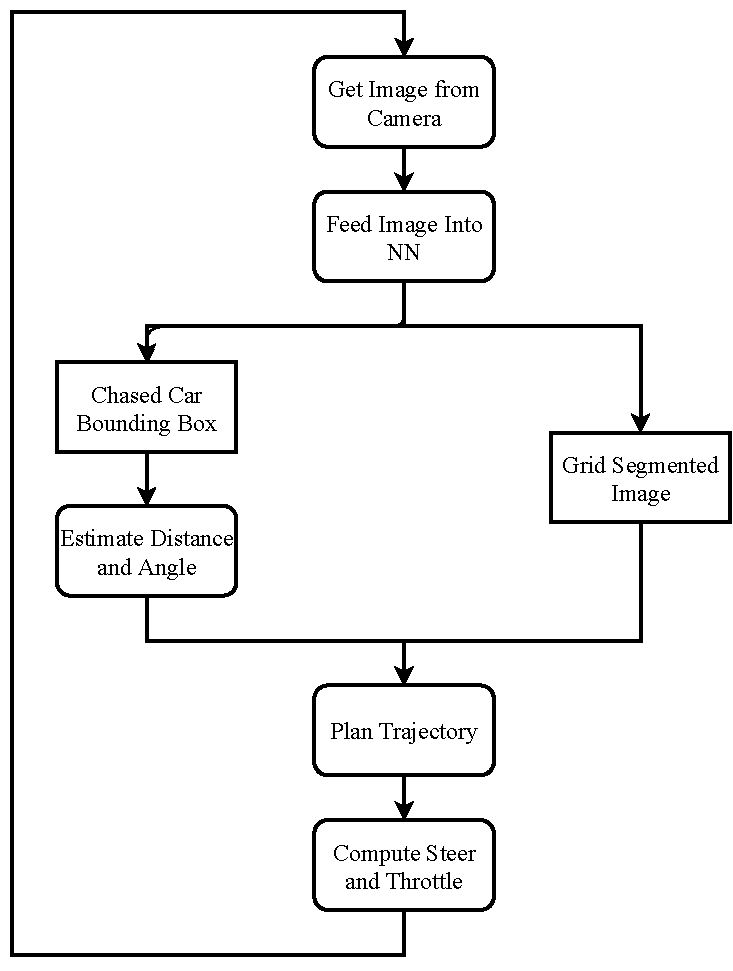
\includegraphics[width=0.7\textwidth]{images/bachelor_diagram4.pdf}
    \caption{Simplified overview of the autonomous driving system}\label{f:overview}
\end{figure}


In the perception part we introduce a novel neural network that detects objects and segments image at the same time. It is able to find a 2D bounding box of the chased car. Furthermore, it segments image into a grid of $S\times S$ cells and makes a classification about each cell whether it's suitable for driving or not. The detection and segmentation is done with a single pass of the image through the neural network. \par

Then, we estimate the angle and distance between the two cars based on the found bounding box of the chased car. In case no bounding box is found we extrapolate the distance and angle. \par

After the perception and localization we plan the trajectory. At this stage we take advantage of the image segmentation. If the conditions allow, we try to drive straight at the last position of the chased car. However if that's not possible, we use the image segmentation and find a direction where it's possible to drive and that is closest to the position of the chased car. \par

Finally, with the trajectory planned, we calculate the steer and throttle to drive the vehicle. We use a PID controller \cite{PID_orig} to control the throttle. It is done by taking into account the current as well as the previous distances between the chasing and chased car. On the other hand, we developed a Pure Pursuit \cite{pure_pursuit_orig} inspired algorithm to control the steering. \par

The details of the method will be described in the following sections.

\section{Computer vision}
\subsection{Dual-task Neural Network}
In this section, we introduce a novel neural network that solves two problems at once - object detection and semantic segmentation. \par

The neural network shares the same backbone for both tasks -- a 53 layer feature extractor called Darknet-53 \cite{YOLOv3}. On top of feature extractor are two sets of layers -- one that gives the output for the object detection and the second that gives an output for the image segmentation. \par

The main idea is in the training of the network. During training, when the network receives training batch of data for semantic segmentation, the output for the object detection is ignored and consequently only the shared layer and the segmentation layers are trained. Equivalently, when the network gets a batch containing object detection data, it updates the weights only on the shared layers and the detection layers. Therefore, the neural network uses two loss functions depending on the batch. \par

During inference, the network works as follows. It is given an image, which passes through the network just once. From this, we get a object detection output as well as the semantic segmentation output. This means that while the training is slightly slower than training a single-task neural network, it is essentially just as fast during inference. \par

For the purpose of autonomous driving the neural network architecture has many advantages over using two separate networks. First, as it was mentioned, it is much faster. That is crucial when driving autonomously, because we want to process as many frames per second as possible and have a fast reaction times to ultimately prevent accidents and crashes. Second, it uses less memory, because most of the network weights are shared. This can be also beneficial for the overall speed since more RAM is available, less disk swapping is required. Finally, it makes integration of the detection and segmentation into our autonomous RC car system a lot simpler.




\subsection{Bounding Box Detector}
In our work, a bounding box is the smallest box which encloses all pixels belonging to the chased RC car in an image. It is also axis-aligned and two dimensional. The detection is performed by a convolutional neural network \cite{CNN_Lecun} with a YOLOv3 neural network architecture \cite{YOLOv3}. \par 
The first version of the YOLO pubslihed in 2015 \cite{YOLO}, made an incredible improvement to the previous state-of-the-art object detection solutions with it's ability to predict bounding boxes of multiple object classes with incredible interference speed. It does so by reasoning globally about the whole images and all its object classes. \par
\begin{figure}[h!]
    \centering
    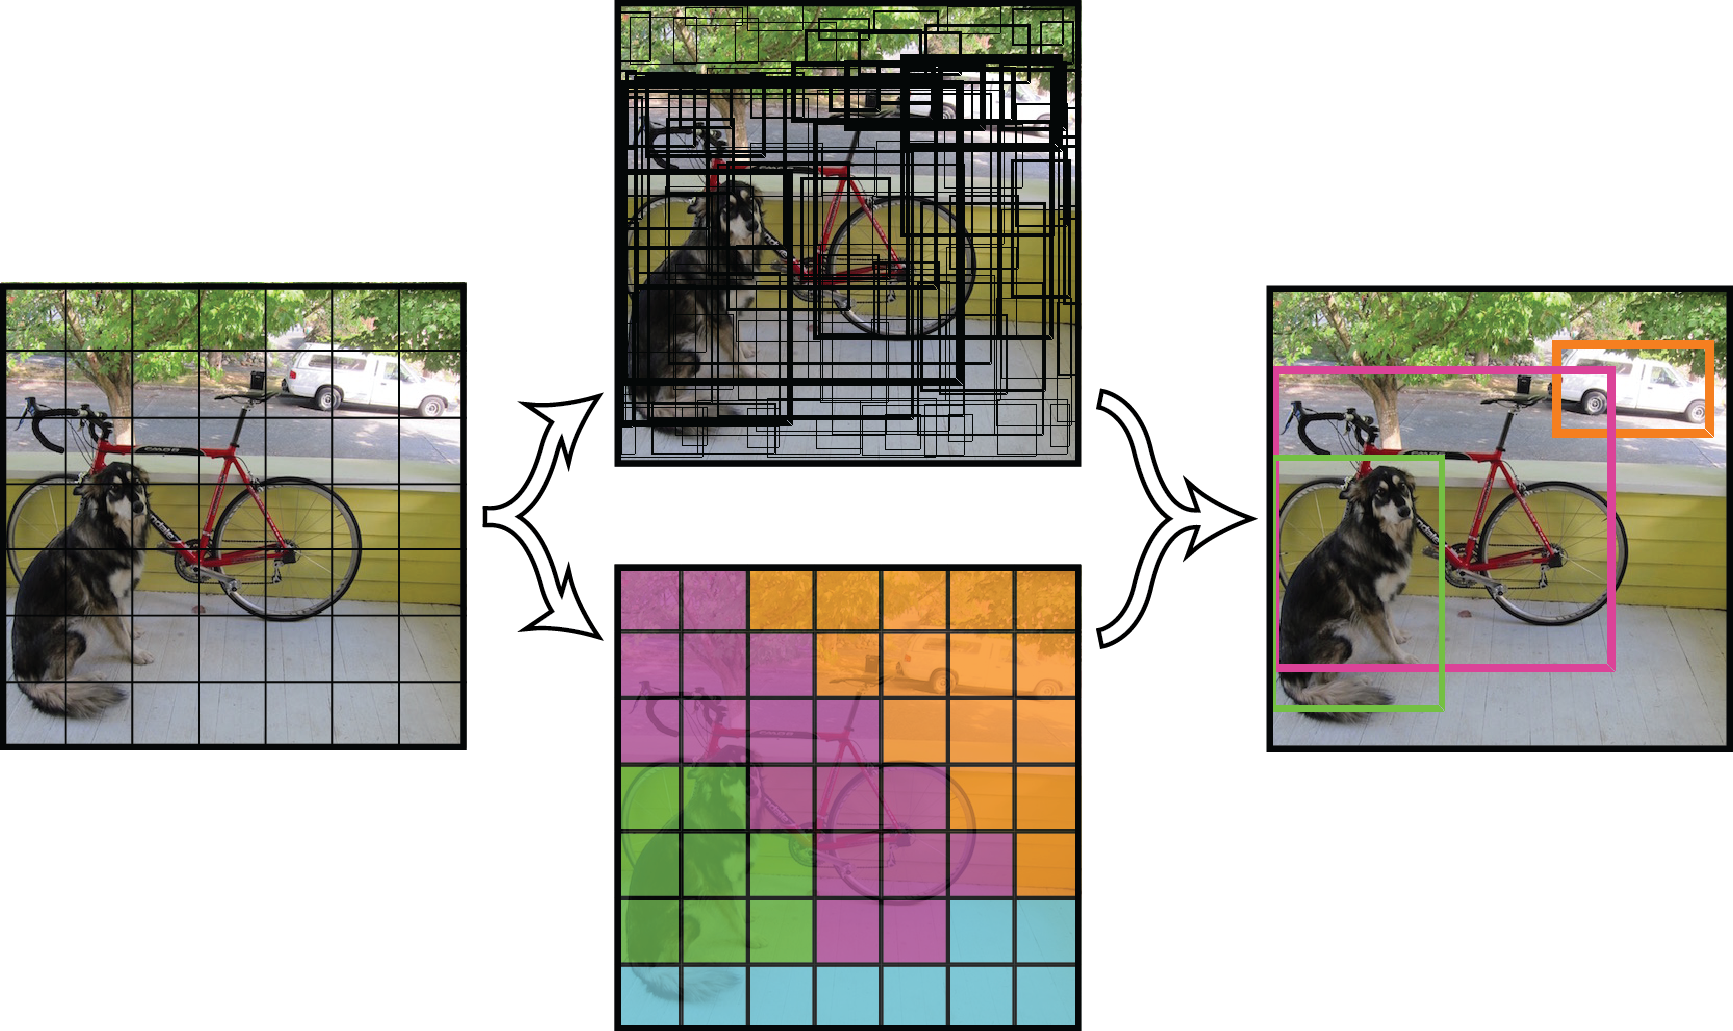
\includegraphics[width=0.8\textwidth]{images/YOLO.png}
    
    \caption{Diagram showing YOLO neural network mechanism, adopted from \protect\cite{YOLO}}\label{f:YOLO}
\end{figure}

The YOLO neural network works by dividing an image into $S\times S$ grid of cells. Each cell makes $K$ bounding box predictions. For each object in the image, the cell that has the center of the object inside is responsible for predicting the bounding box for said object. This can be seen in the top middle image in the Figure \ref{f:YOLO}. Separately, each cells outputs $C$ values where each value represents a predicted probability whether object from a class $C_i$ is in the cell. The resulting class map from these predicted probabilities can be seen in the bottom middle image in the Figure \ref{f:YOLO}. 
%TODO how the backpropagation works
\par
Two years after introducing YOLO, the second version of called YOLO9000 \cite{YOLO9000} was introduced.  In the first version of YOLO, each cells makes $K$ bounding box predictions of a random size resulting in steep gradient changes during training. %(TODO - my own words)
This is improved in YOLO9000 by calculating the expected bounding box sizes by clustering the bounding boxes of the training set. These expected bounding boxes are called anchors or priors. It also uses different network architecture called Darknet-19 and enables detection on different image sizes. \par
% TODO add ""

The third version of the YOLO architecture improves YOLO in two main way. Firstly, it adds more layers to the Darknet network architecture. Secondly, inspired by Feature Pyramid Networks \cite{FPN}, it predicts boxes at 3 different scales. To be specific, instead of dividing the image into $S\times S$ grid of cells, YOLOv3 divides it into $S\times S$, $(S\cdot2)\times (S\cdot2)$ and a $(S\cdot4)\times (S\cdot4)$ grid of cells.
%This is then used to... TODO


\subsection{Angle and Distance Estimation}
One of the most crucial information when chasing another vehicle is it's relative angle and distance to the chasing car. In our work, we are trying to estimate the angle between the normal vector of a camera on the chasing car (in the direction of the car) and the vector pointing from the camera to the center of the back of the pursued car. Furthermore, we want to estimate the distance between the two cars. To be specific, the distance between the front of the chasing car and the center of the back of the pursued car.

\begin{figure}[h!]
    \centering
    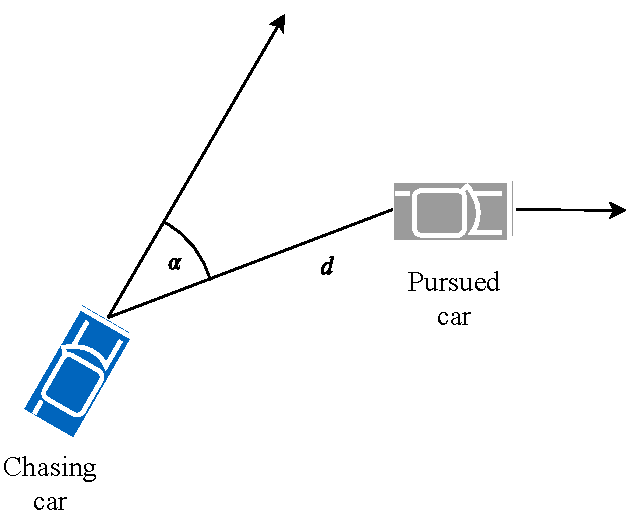
\includegraphics[width=0.7\textwidth]{images/chasing_diagram.pdf}
    
    \caption{Diagram showing blue chasing car on the left and pursued car on the right. It shows the ground truth distance $d$ and the angle $\alpha$ we are trying to estimate }\label{f:chasing_diagram}
\end{figure}

The Figure \ref{f:chasing_diagram} shows this problem in a simplified 2D view. To estimate the distance and the angle of the car from an image, we took advantage of existing solutions solving PnP (Perspective-n-Point) problem. PnP is a problem of estimating position and orientation of a camera from a set of $n$ 3D points, their corresponding 2D projections in the image and the calibrated intrinsic camera parameters. This leads us to an equation 
\begin{equation}
s\,p_{image} = K\,[\,R\, |\, T\, ]\, p_{world}
\end{equation}
, where $p_{image}$
are the coordinates of the points in the image, $p_{world}$ are the corresponding world coordinates, $K$ is the matrix of intrinsic camera parameters and $R$ and $T$ are the rotation and translation we are calculating. Here is the full equation: 


\begin{equation}
s\begin{bmatrix}u\\v\\1\end{bmatrix} = \begin{bmatrix}
f_x & \gamma & u_0\\
0 & f_y & v_0\\
0 & 0 & 1
\end{bmatrix}\begin{bmatrix}
r_{11} & r_{12} & r_{13} & t_{1}\\
r_{21} & r_{22} & r_{23} & t_{2}\\
r_{31} & r_{32} & r_{33} & t_{3}\\
\end{bmatrix}
\begin{bmatrix}x\\y\\z\\1\end{bmatrix}
\end{equation}

In our case, the image points $p_{image}$ are the bounding box corners of the detected car. We can also estimate the world coordinates $p_{world}$ by measuring the width and height of the chased RC car. Finally, the the intrinsic camera parameters such as focal lengths $f_x$ and $f_y$ were calculated based on official documentation from the ZED camera. Then, we plug these values into a OpenCV \cite{opencv_library} library function which gives us the translation and rotation vectors. Afterwards, we calculate the desired estimated distance by calculating euclidean distance between the translation vector and the origin. Similarly, we extract the desired estimated angle by calculating arc tangent of the rotation vector. 

Finally, since we are using a stereo camera and the camera lens which was used is not in the center of the front of the car, we have convert the calculated angle and distance as if the camera was in the center of the front of the car. We achieve this by simple triangulation.

\subsection{Angle and Distance Extrapolation}
In the previous section, we have described how we estimate angle distance based on bounding box of the chased car. However, in some cases the detector is unable to detect object in the image due to poor light conditions in the scene, or because the pursued vehicle is only partially vehicle due to some object blocking it. Furthermore, there are cases when the chased car is not in the image at all. In these cases we need to make a reasonable prediction about the position of the chased car. \par


We extrapolate the angle and the distance of the chased car based on the previous estimations. At the heart of the extrapolation algorithm is exponential moving average. In fact, we use just six variables to store the information about the whole history of estimated angles and distances. The idea will explained on extrapolating distances. The angle extrapolation is done similarly. \par
The whole extrapolation revolves around using the following equation:
\begin{equation}
exp = \alpha\cdot d_i + (1-\alpha)\cdot exp
\end{equation}
The $\alpha$ variable is in this case a value in the range [0,1] that sets the weight of the last predicted estimate $d_i$ at frame $i$. In our algorithm, we have chosen value $\alpha=0.5$. The $exp$ variable is the exponential variable where we store the information about the estimation history. At every frame, we update the value of $exp$. \par

If the chased car is detected in the image we set $d_i$ equal to the predicted estimate and update the variable $exp$.
However, if the the chased car is not in the image, or the detection is unsuccessful we use the following simple extrapolation to set the estimated value of $d_i$ equal to:
\begin{equation}
d_i = 2\cdot d_{i-1} - d_{i-2}
\end{equation}
Afterwards, we update the $exp$ value and return it as the predicted estimate in case no bounding box was found in the image. 
\par This method allows us to extrapolate the angle and the distance very fast in a $\mathcal{O}(1)$ time and space complexity with almost no overhead.

\subsection{Image Segmentation}


\section{Control And Planning}
In this section, we will explain how we control steering and throttle of the vehicle based on the extracted information from the camera. Conversely to many algorithms, we control steering and throttle separately. Steering control is inspired by pure pursuit algorithm and throttle is controlled by a PID controlled.


\subsection{Pure Pursuit Inspired Algorithm}
Pure pursuit algorithm is a path tracking algorithm that moves a vehicle from its current position to a some look-ahead position on the path. It was invented in the 1980s as it was used in the first demonstration of an autonomous vehicle capable of following a road using imagery from a black and white camera \cite{pure_pursuit_orig}. The goal of the demonstration was to keep the vehicle centered on the road while it was driving at a constant speed.\par
The algorithm works as follows. Firstly, it finds the goal point on the path. Then, it transforms the goal point to vehicle coordinates and finally it calculates the curvature that will drive the vehicle to the look-ahead position on the path. \par
In our work, we were inspired by the algorithm. As opposed to the pure pursuit algorithm settings, our car doesn't move at a constant speed. Secondly, we are not following a path, but rather chasing a moving RC car. Therefore, every time we process an image from the camera, we update our goal position. But unlike in the path following algorithm, the destination position is updated to the current position of the chased RC car rather than to a position on a path. \par
Conversely to the pure pursuit algorithm, we also don't calculate the curvature to control the steering. That is because we need to update our the steering every frame based on the position of the chased RC car and take more aggressive turns to chase the pursued vehicle. In our algorithm we calculate the steering value with the following function:

\begin{equation}steer = (\cfrac{\alpha}{\textrm{180}})^{2}\end{equation}

The value $\alpha$ represents the angle between the chasing and the chased car shown in the Figure \ref{f:chasing_diagram}. The $steer$ variable is a value in the [-1, 1] range, where -1 and 1 represent the highest left-turn and right-turn steering angle the car can make respectively. We square the result of the division, because the steering control on the RC car is non-linear. We don't square the divison in the CARLA simulation.

% we dont use curvature because... update position often.. 
\subsection{PID Controller}

\chapter{Experiments}

\section{Vehicle Detection}
\subsection{Dataset}
In order to train and evaluate 2D object detector capable of creating 2D bounding box around the chased RC car in a image, a dataset was needed. The collected dataset consists of \textbf{440} annotated images. All image annotations are in the PASCAL VOC data format introduced in the PASCAL Visual Object Classes Challenge \cite{pascal-voc}. Each image has it's annotation that contains pixel coordinates of the bounding box corners for each object in the image. In our dataset, only one object per image is annotated -- the chased RC car. The data were collected from multiple locations around Czechia and also under different lighting conditions. The majority of images were collected by the ZED Stereo camera attached to the chasing RC car. 


\subsection{Detection Results}
The collected dataset was split into three sets. The majority of 80\% of the images were randomly selected into training set, 10\% were randomly selected into validation set and the remaining images were used as a testing set. To evaluate the model, we calculated multiple values -- recall, precision, XY loss and WH loss. To understand recall and precision we need to first define IoU (Intersection over union). IoU measures how much the predicted bounding box overlaps with the ground truth (annotated bounding box). It is defines as 
\begin{equation}IoU = \cfrac{\textrm{Area of overlap}}{\textrm{Area of union}}\end{equation}

When calculating precision and recall, we say that the predicition is either true positive or false positive when IoU is bigger than $0.5$. XY loss is calculated as a mean squared error (MSE) between the center of the predicted bounding box and the center of ground truth bounding box. WH loss on the other hand is the difference between width and height of the predicted bounding box and the ground truth bounding box. When calculating both of these values, coordinates and image dimensions have been scaled to the [0, 1] range. \par
The model has been trained to minimize sum of the XY and WH losses. During training, the model with the lowest loss on the validation dataset has been saved.

\begin{table}[]
\begin{tabular}{l|llll}
\hline
            & Precision & Recall & XY loss & WH loss \\ \hline
Testing set & 99.8\%    & 97.7\% & 0.066   & 0.227   \\ \hline
\end{tabular}
\label{tab:detection}
\caption{Evaluation of the detector on a testing set}
\end{table}



\begin{figure}[h!]
    \centering
    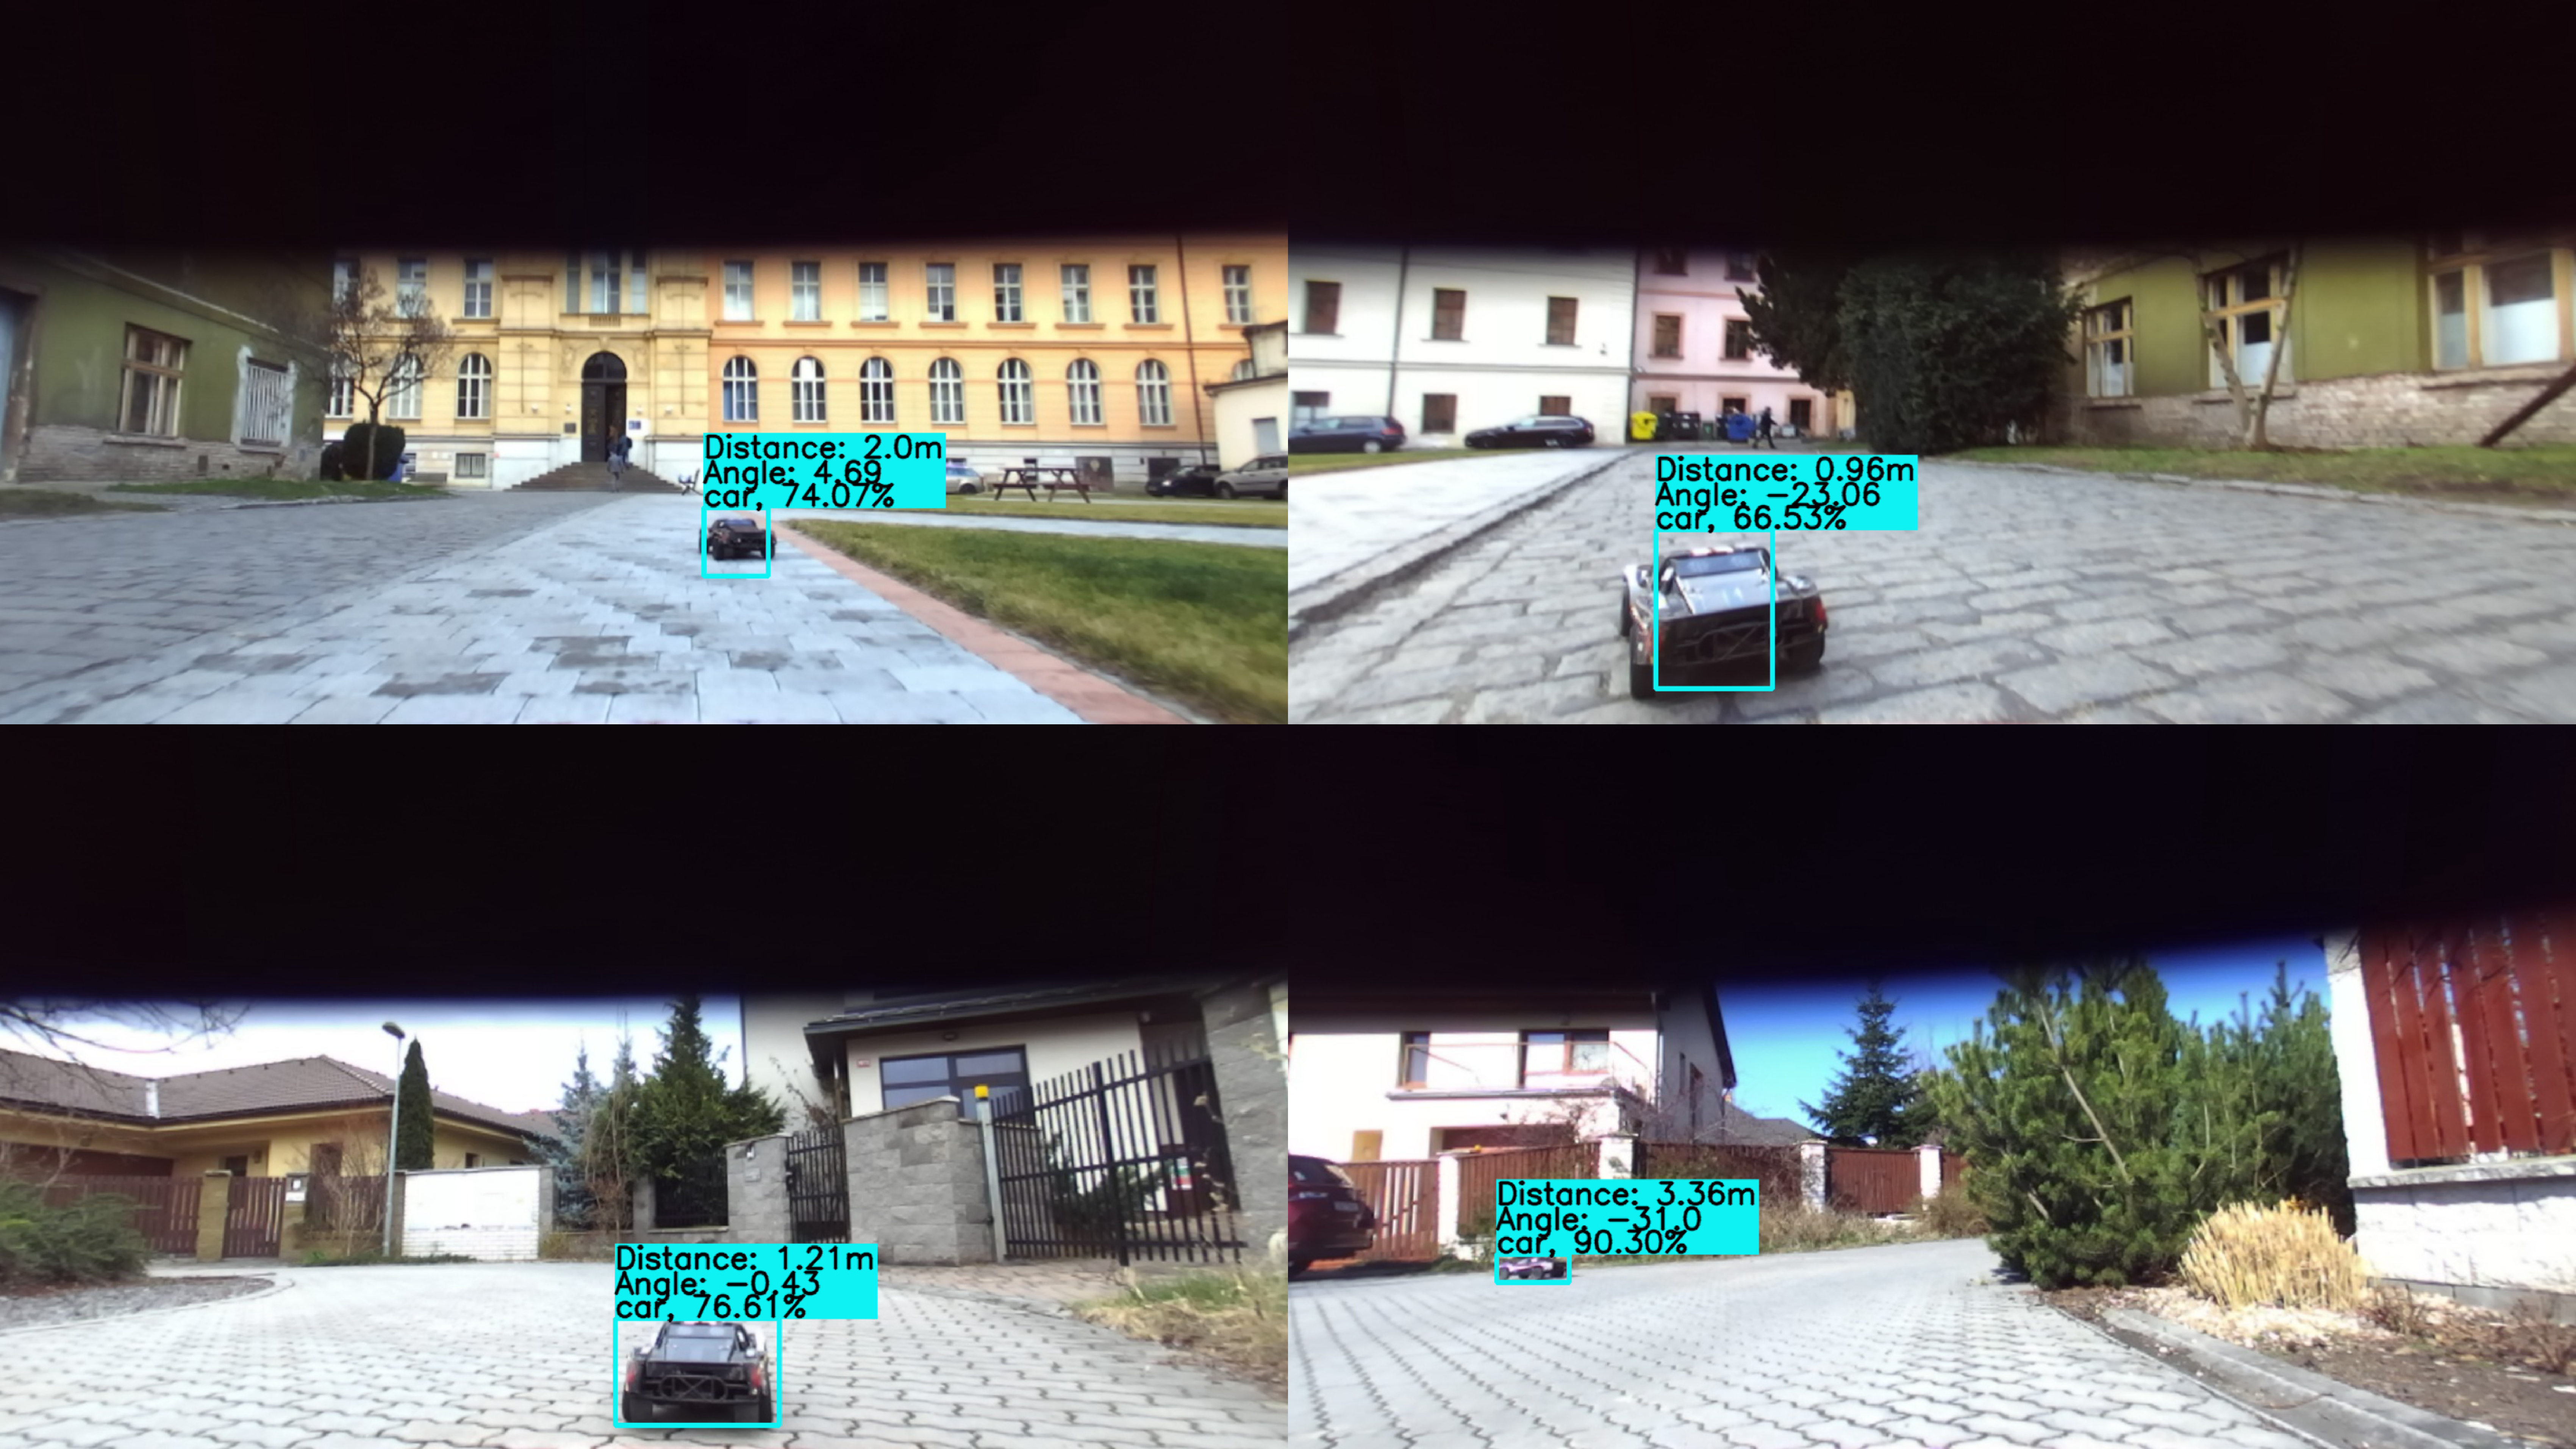
\includegraphics[width=1\textwidth]{images/Collage_detection(1).pdf}
    
    \caption{Detection, distance and angle estimation performed on images from the RC car camera. The images are part of the collected dataset}\label{f:detection_images}
\end{figure}

\section{Simulation}
\subsection{CARLA Environment}
\subsection{Experiment Setup}
\subsection{Results}

\section{Real-world Testing}
\subsection{RC Cars Description}
\subsubsection{Chasing RC car}
For the deployment of our autonomous chasing algorithm a sub-scale vehicle platform called Toyota Mini (ToMi) was used %TODO cite. 
The platform is built around a large 1:5 scale RC car "Losi Desert Buggy XL-E 4WD". This electrically powered car has 0.9 x 0.5 meters length and width dimensions with reported maximal speed of up to 80km/h. At the core of the platform is a Raspberry Pi with a Navio-board that generates pulse width modulation signals for the throttle and steering to the servomotor. It is also equipped with a ZED stereo camera for taking color images, NVIDIA Jetson AGX Xavier graphics card for image processing and neural network interference. Finally, it is equipped with SSD to provide additional storage, GPS and IMU. \par
The whole simplified process flow is as follows. First, an image is taken by camera, which then goes to graphics card where it's analyzed by our algorithm. Then, based on the image analysis a steer and throttle values are updated. These values are transmitted from the graphics card to the Raspberry Pi which then sends signal to the servomotor that controls the vehicle.

\subsubsection{Chased RC car}
The RC car used as the chased vehicle is a 1:10 scale "Losi XXX-SCR RTR". This electrically powered car has 0.55 x 0.29 meters length and width dimensions with reported maximal speed of up to 55 km/h.

\begin{figure}[h!]
    \centering
    \subfloat[Inside of the chasing RC car]{{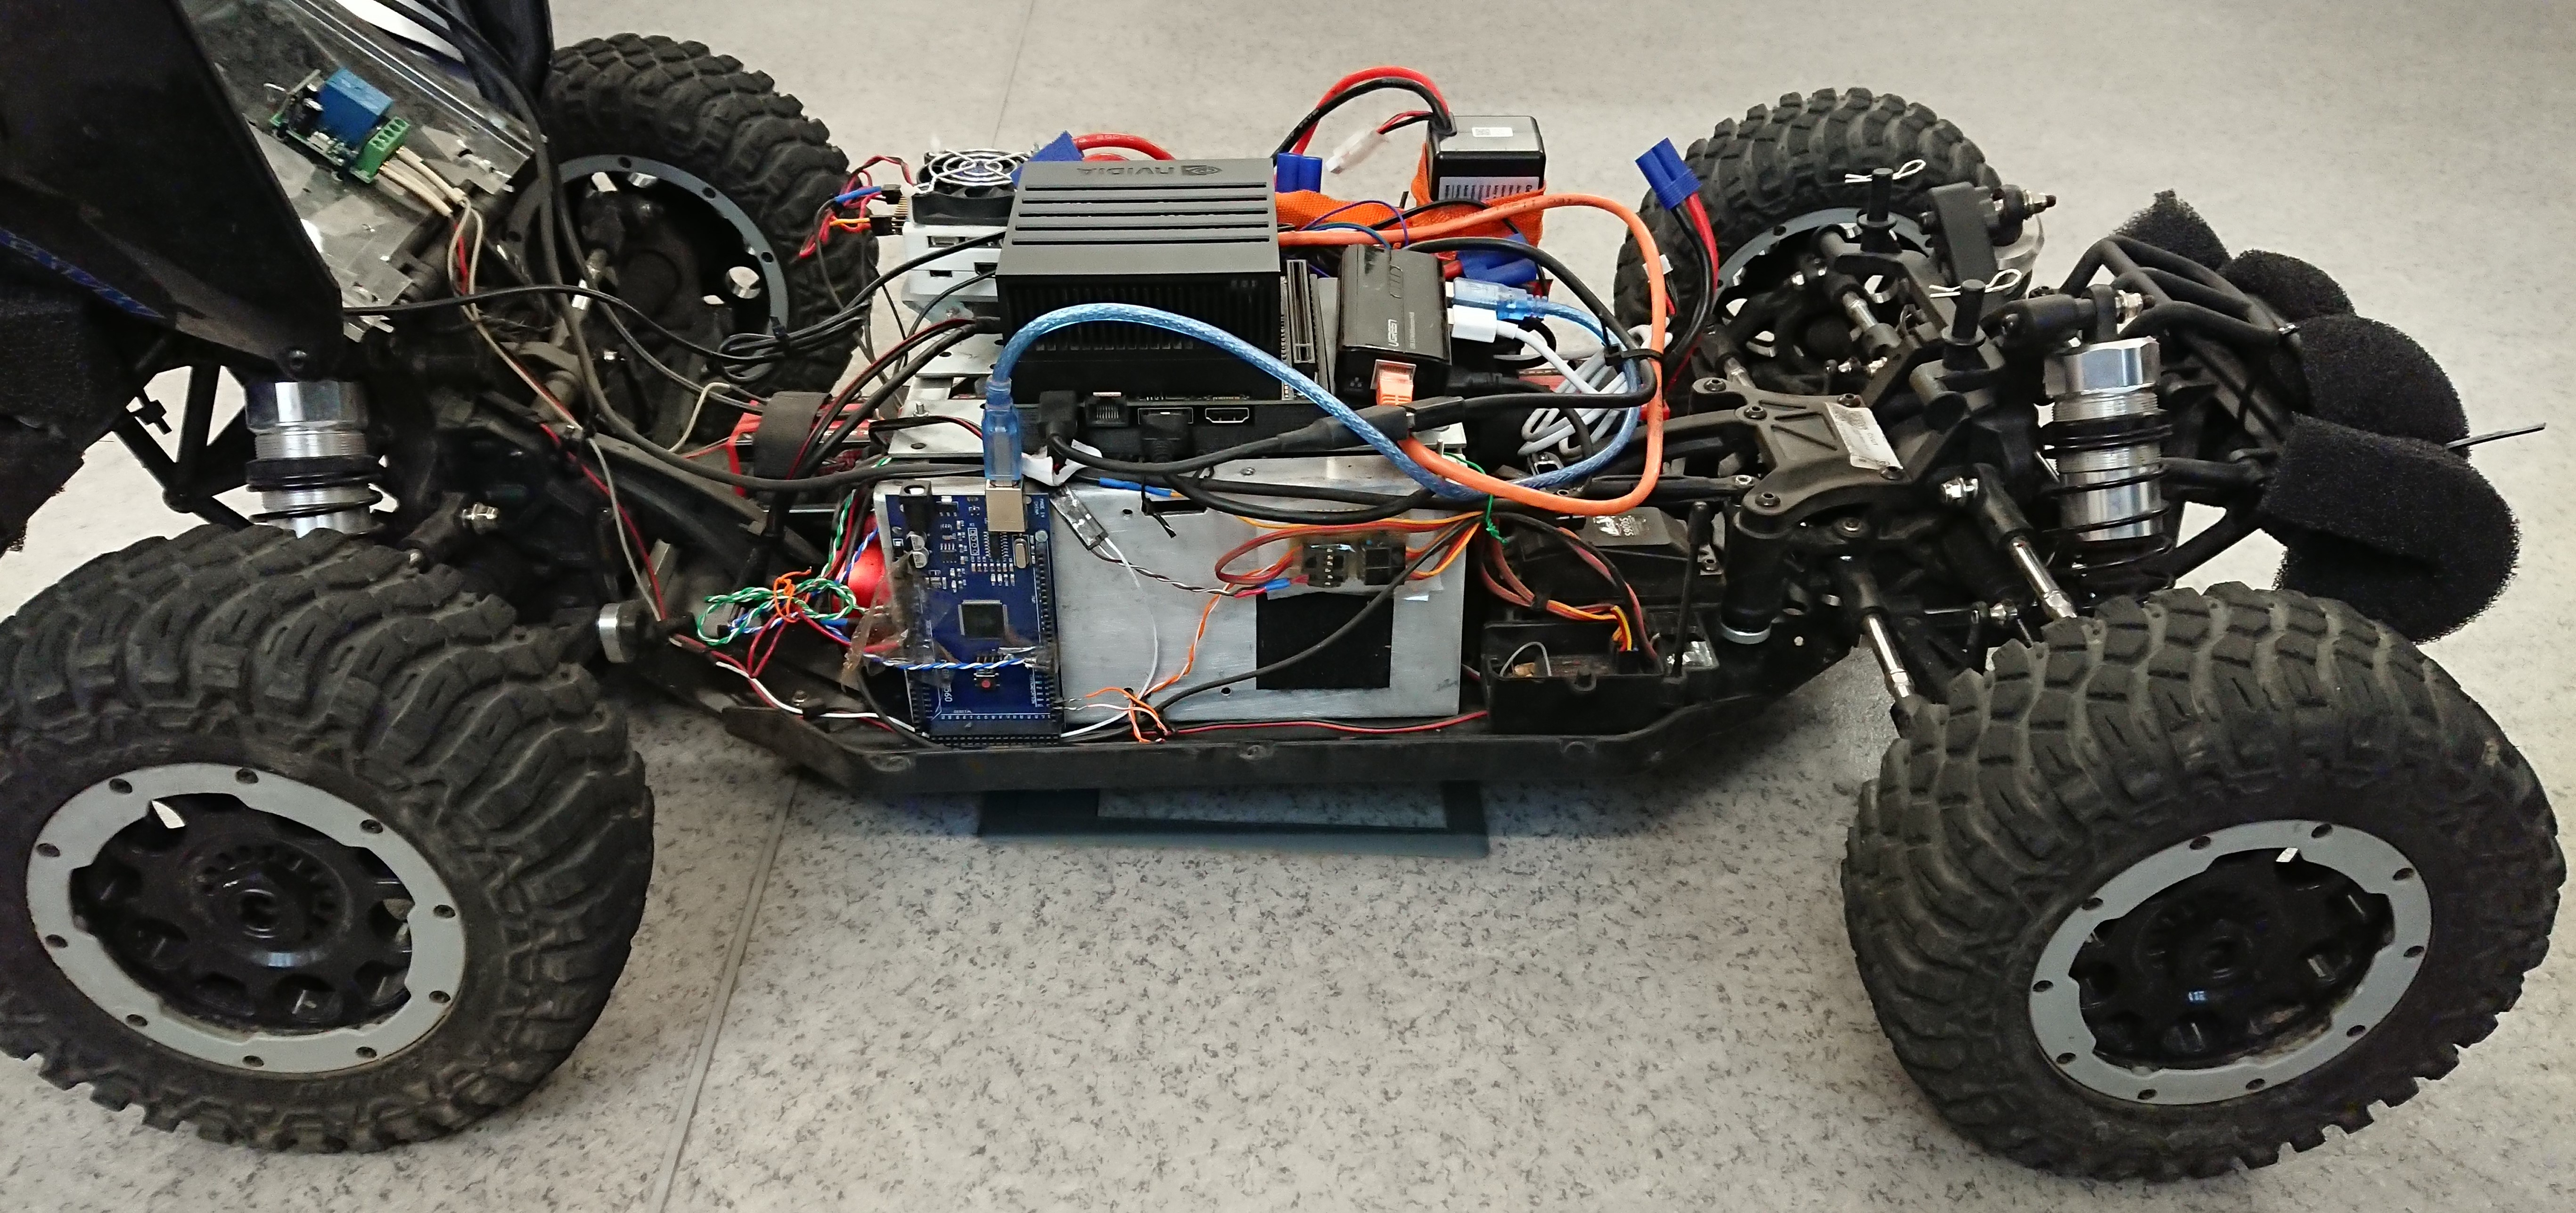
\includegraphics[height=3.7cm]{images/inside.jpg} }}%
    \qquad
    \subfloat[Chasing RC in the back and the chased RC car in the front]{{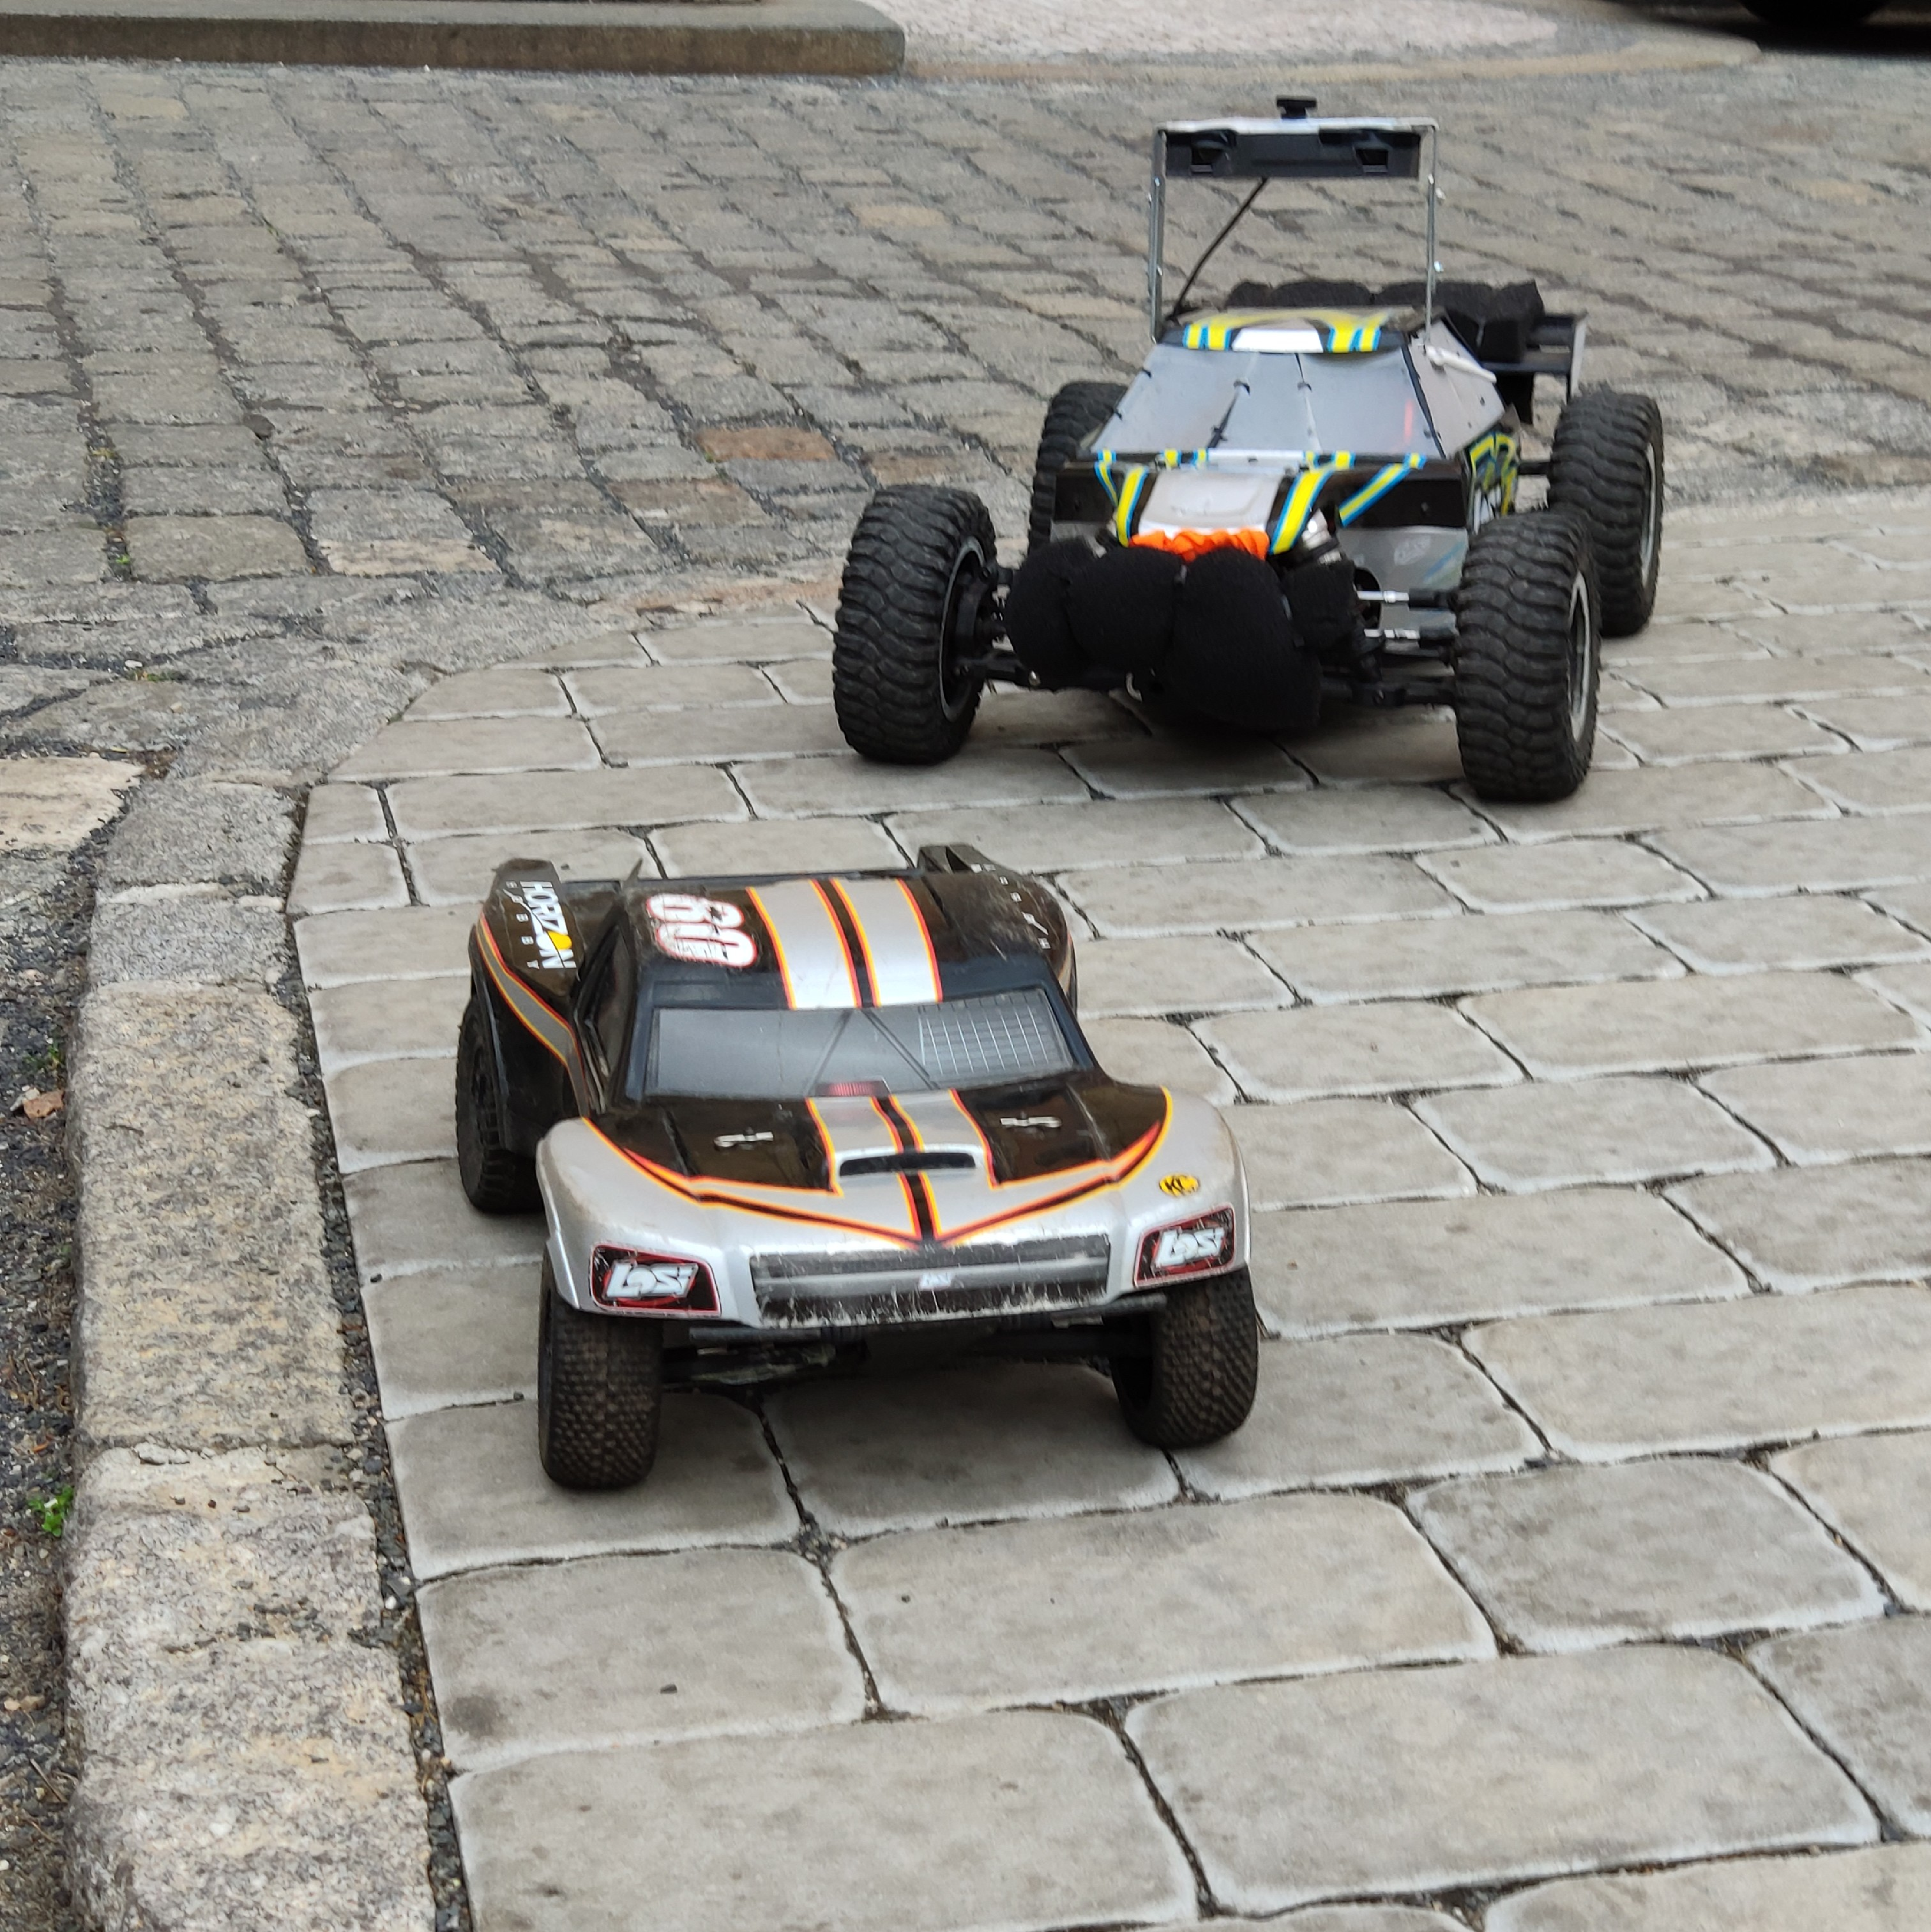
\includegraphics[height=3.7cm]{images/rc_cars.pdf} }}%
    \caption{Hardware inside of the autonomous chasing RC car on the left and both RC cars used for testing on the right}%
    \label{fig:rc_cars}%
\end{figure}

%\begin{figure}[h!]
%\centering
%\begin{subfigure}{.5\textwidth}
%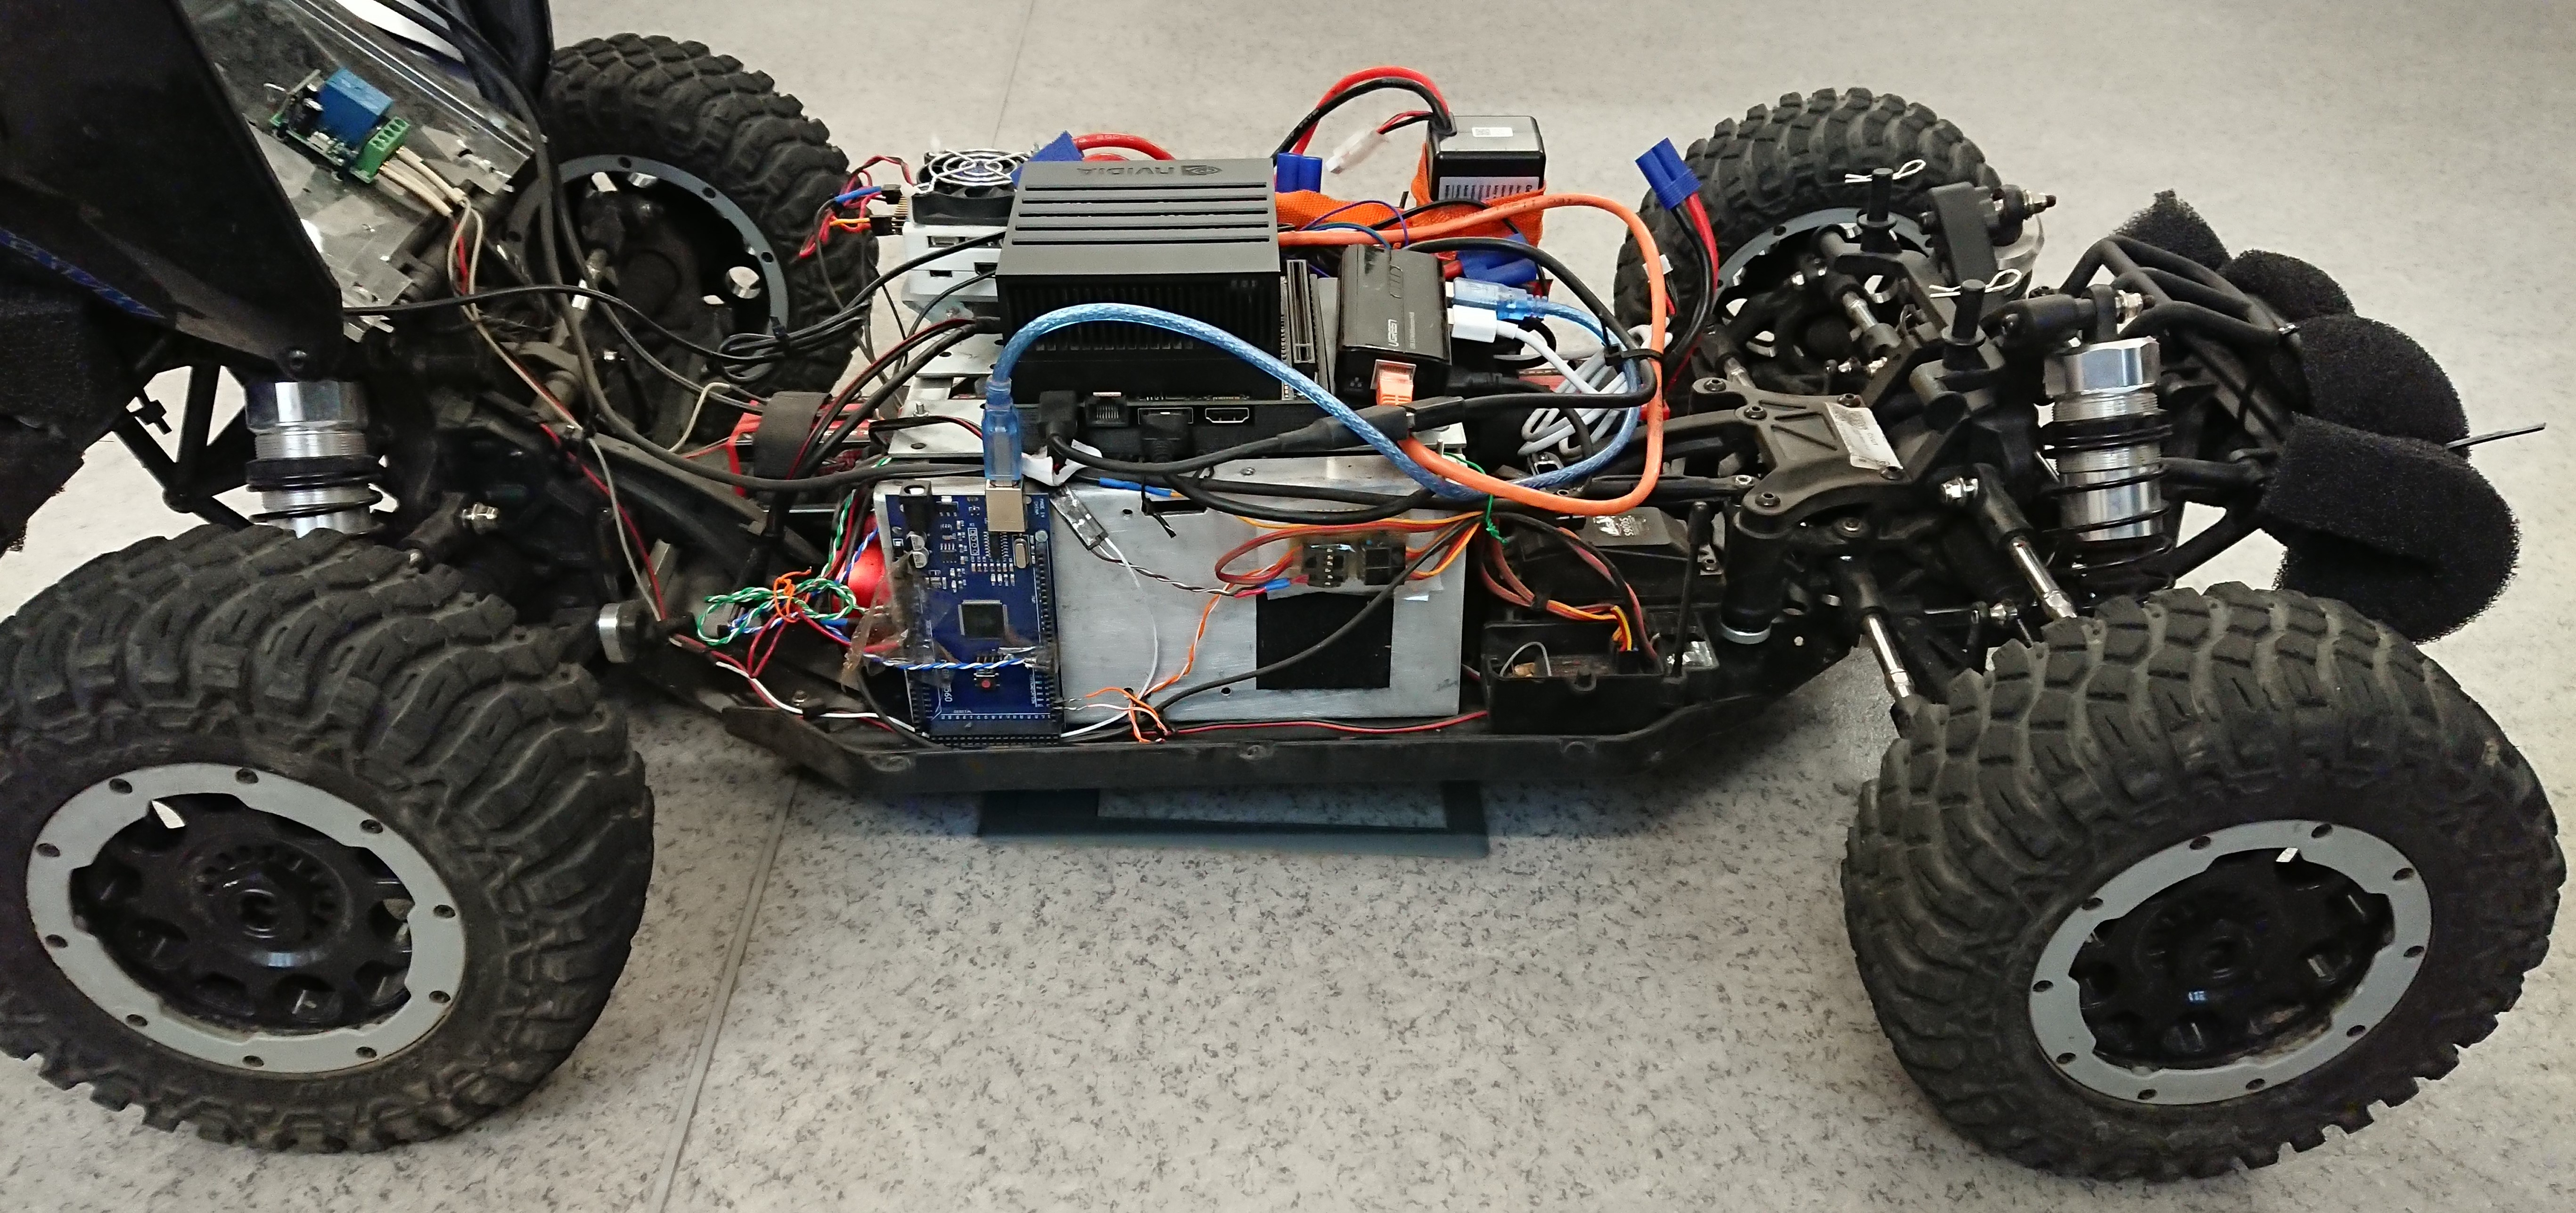
\includegraphics[width=.4\linewidth]{images/inside.jpg}
%\end{subfigure}
%\begin{subfigure}{0.5\textwidth}
%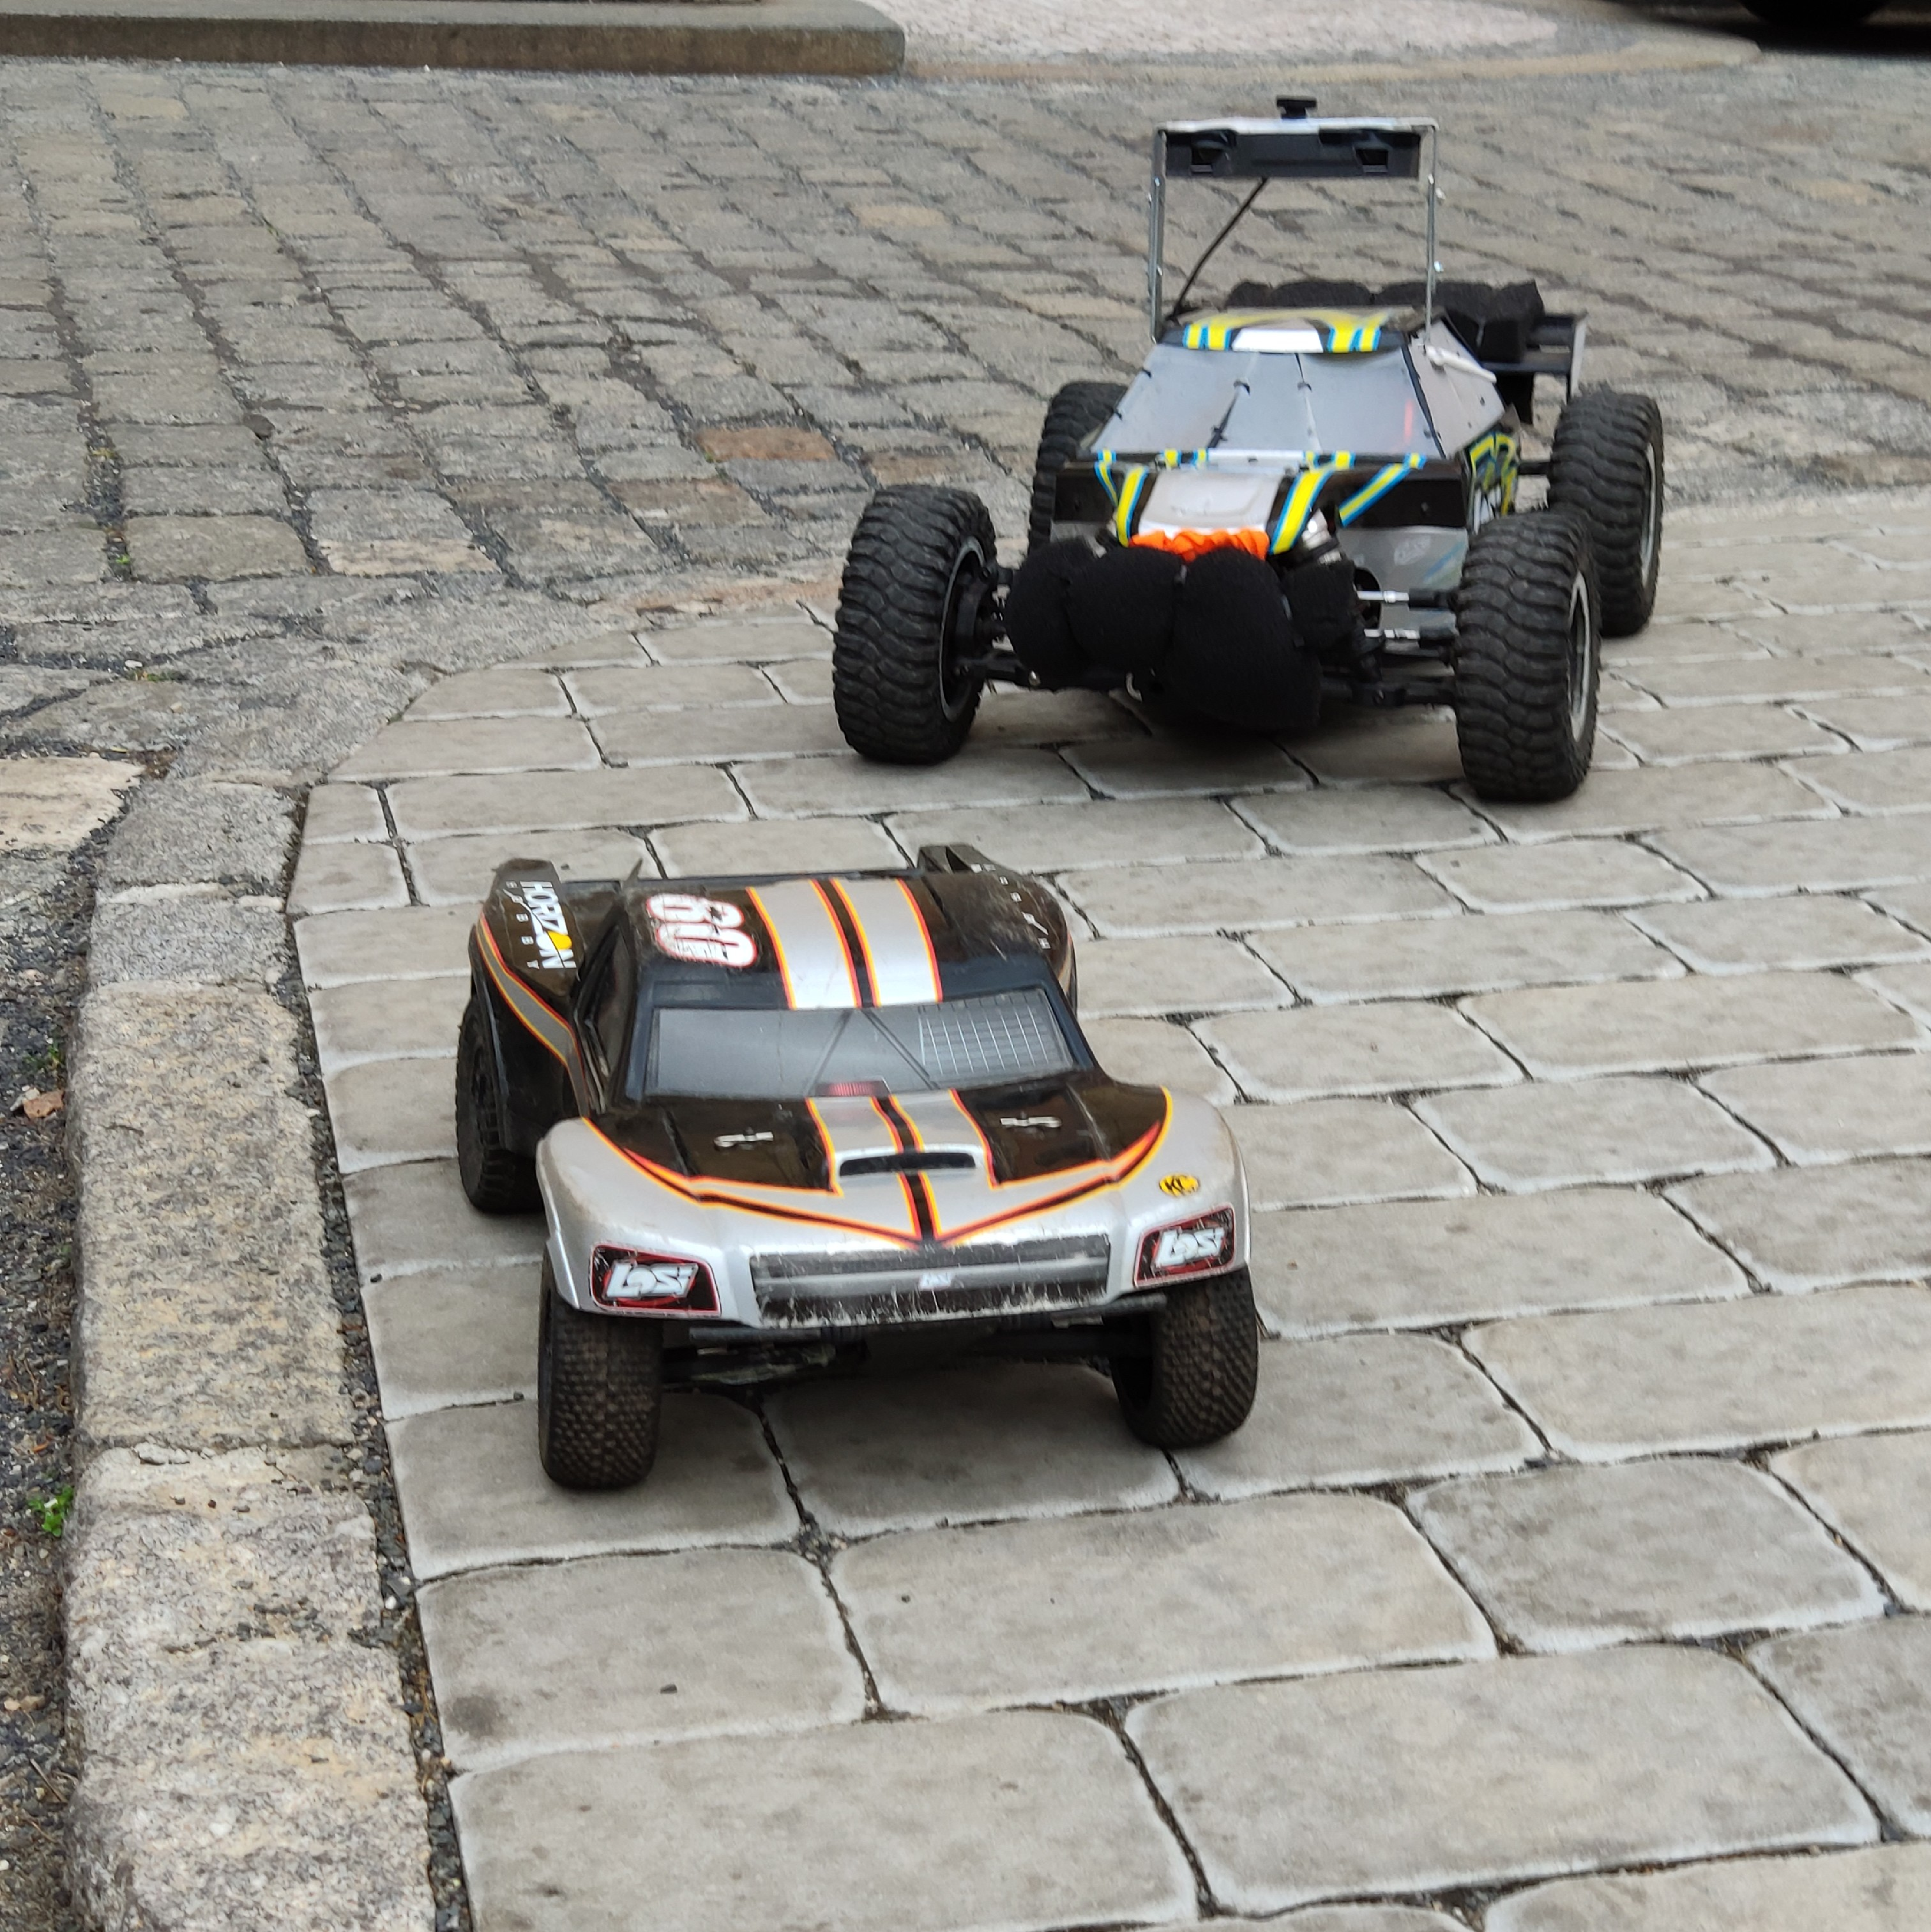
\includegraphics[width=.4\linewidth]{images/rc_cars.pdf}
%\end{subfigure}
%\caption{Both RC cars used for testing. The autonomous chasing car is in the back, while the manually driven car used as the pursued %car is in the front}
%\end{figure}


\subsection{Experiments}



\chapter{Conclusion}

\bibliography{citations}
\bibliographystyle{IEEEtran}

\end{document}

